\documentclass{beamer}
\usepackage{graphics}
\usepackage{epsfig}
\usepackage{multicol}
\usepackage{pifont}
\setbeamertemplate{navigation symbols}{}
\newcommand{\RR}{\ensuremath{\mathbb{R}}}
\newcommand{\NN}{\ensuremath{\mathbb{N}}}
\newcommand{\QQ}{\ensuremath{\mathbb{Q}}}
\newcommand{\CC}{\ensuremath{\mathbb{C}}}
\newcommand{\ZZ}{\ensuremath{\mathbb{Z}}}
\newcommand{\TT}{\ensuremath{\mathbb{T}}}
\newcommand{\HH}{\ensuremath{\mathbb{H}}}
\DeclareMathOperator{\Min}{Min}
\DeclareMathOperator{\Dom}{Dom}
\DeclareMathOperator{\vol}{vol}
\DeclareMathOperator{\Aut}{Aut}
\DeclareMathOperator{\Stab}{Stab}
\DeclareMathOperator{\Sym}{Sym}
\DeclareMathOperator{\Grp}{Grp}
\DeclareMathOperator{\HYP}{HYP}
\DeclareMathOperator{\CUT}{CUT}
\DeclareMathOperator{\GL}{GL}
\DeclareMathOperator{\AGL}{AGL}
\DeclareMathOperator{\Id}{Id}
\DeclareMathOperator{\mint}{min}
\DeclareMathOperator{\vertt}{vert}
\DeclareMathOperator{\conv}{conv}
\DeclareMathOperator{\rank}{rank}
\DeclareMathOperator{\divt}{div}

\def\QuotS#1#2{\leavevmode\kern-.0em\raise.2ex\hbox{$#1$}\kern-.1em/\kern-.1em\lower.25ex\hbox{$#2$}}

\begin{document}
\title{A two-way Coupling of the Adriatic sea Circulation and wave models}
\author{
\begin{center}
\textcolor{red}{\large \underline{Dutour Sikiri\'c M.}}$^{(1)}$
\textcolor{red}{\large Roland A.}$^{(2)}$
\textcolor{red}{\large Kuzmi\'c M.}$^{(1)}$
\textcolor{red}{\large Janekovi\'c I.}$^{(1)}$
\textcolor{red}{\large Toma\u zi\'c I.}$^{(1)}$\\[2mm]
\end{center}
\begin{flushleft}
(1) \textcolor{blue}{Rudjer Bo\u skovi\'c Institute, Croatia}\\[2mm]
(2) \textcolor{blue}{Technische Universit\"at Darmstadt, Germany}
\end{flushleft}
}
\date{\today} 
\frame{\titlepage} 


%\author{
%{\small
%\begin{center}
%\textcolor{red}{\large Mathieu Dutour Sikiri\'c}\\[2mm]
%\textcolor{red}{Rudjer Boskovic Institute, Croatia}
%\textcolor{red}{\large Aron Roland}\\[2mm]
%\textcolor{red}{Institut of Hydraulic Engineering, Darmstadt}\\[2mm]
%\textcolor{red}{\large Igor Toma\u zi\'c}\\[2mm]
%\textcolor{red}{Rudjer Boskovic Institute, Croatia}
%\textcolor{red}{\large Ivica Janekovi\'c}\\[2mm]
%\textcolor{red}{Rudjer Boskovic Institute, Croatia}
%\textcolor{red}{\large Milivoj Kuzmi\'c}\\[2mm]
%\textcolor{red}{Rudjer Boskovic Institute, Croatia}
%\end{center}
%}
%}







%\frame{
%  \frametitle{Stochastic wave modelling}
%\begin{itemize}
%\item Oceanic models are using grids (structured or unstructured) of size $1km\leq d\leq 10km$ to simulate the ocean
%\item But oceanic waves have a typical wavelength $2m$ $\leq$ $L$ $\leq$ $100m$. So, we cannot resolve waves in the ocean.
%\item We write the linear dispersion relations as:
%\begin{equation*}
%\sigma^2 = g k tanh(kh) \mbox{~and~} \omega = \sigma + {\bf k}\cdot {\bf u}
%\end{equation*}
%\item But if one uses phase averaged models and uses stochastic assumptions then it is possible to model waves by a spectral wave action density
%$N({\bf x},{\bf k})$
%\item This density satisfies a Wave Action Equation (\textcolor{red}{WAE}) which represents advection, refraction, frequency shifting and source terms:
%\begin{equation*}
%\begin{array}{c}
%\frac{\partial N}{\partial t} + \nabla_x(({\bf c}_g+{\bf u}_A)N) + \nabla_k(\dot{k} N) 
% + \nabla_{\theta}(\dot{\theta} N) = S_{tot}\\
%S_{tot} = S_{in} + S_{nl3} + S_{nl4} + S_{bot} + S_{ds} + S_{break} + S_{bf}
%\end{array}
%\end{equation*}
%with $u_A$ being the surface current.
%\end{itemize}
%}




%\frame{
%  \frametitle{Doppler shift}
%\begin{itemize}
%\item Suppose that we have a uniform current ${\bf u}$ then the dispersion relation is changed to
%\begin{equation*}
%\sigma^2 = g k  \tanh( kh) \mbox{~and~} \omega = \sigma + {\bf k}\cdot {\bf u}
%\end{equation*}
%with $\sigma$ the intrinsic frequency and $\omega$ the absolute frequency.
%\item In the case of a sheared current, the Doppler shift relation changes to
%\begin{equation*}
%\omega = \sigma + {\bf k}\cdot\int_{z=-h}^{z=\xi} {\bf u} \frac{2k\cosh(2k(z+h))}{\sinh(2kD)} dz
%\end{equation*}
%\item The advection velocity ${\bf u}_A$ is usually approximated by the surface current velocity. There is unfortunately no Wave Action Equation in the case of sheared currents.
%\end{itemize}
%}

\frame{
  \frametitle{Outline}

\begin{enumerate}
\item[\textcolor{red}{(1)}] Motivation and goals
\item[\textcolor{red}{(2)}] Models setup \& coupling
\item[\textcolor{red}{(3)}] Wind forcing and validation
\item[\textcolor{red}{(4)}] Simulations and comparison to ADCP measurements
\item[\textcolor{red}{(5)}] Summary and outlook
\end{enumerate}
}


\frame{
  \frametitle{\textcolor{red}{(1)} Motivation and goals}
\begin{itemize}
\item Long term goal: two-way coupled system (WRF - ROMS - WWMII)
\item Current focus: coupling circulation and wave models, and related wind forcing.
\end{itemize}

%\begin{itemize}
%\item We are interested in the Adriatic response to strong wind.
%\item The wave effects are expected to be important.
%\end{itemize}

\begin{center}
\begin{minipage}[b]{5.3cm}
%l b r t
%\resizebox{5.2cm}{!}{\includegraphics[trim=35mm 11mm 35mm 11mm, clip]{PictureElect/BathymetryRiver.png}}\par
%\resizebox{5.2cm}{!}{\includegraphics{FIG_wave/AdriaticMap.png}}\par
\resizebox{5.2cm}{!}{\includegraphics{NADWEX/2009-01-25-VK-02.jpg}}\par
%\resizebox{5.5cm}{!}{\includegraphics[bb=101 32 477 403, clip]{PictureElect/BathymetryRiver.pdf_V1}}\par
\end{minipage}
\begin{minipage}[b]{5.3cm}
Two dominant winds
\begin{itemize}
\item Bora: cold and dry cross-basin, north-easterly wind
\item Sirocco: warm, along-basin, long fetch, southerly wind
%\item Significant inflow/outflow occurs at the Ottranto strait and generates the highest tides of the Mediterranean.
\end{itemize}
Both impact waves and circulation fields.
\end{minipage}
\end{center}

}





\frame{
  \frametitle{\textcolor{red}{(2)} The {\tt ROMS} model and {\tt WWM-II} model}
The \textcolor{red}{Regional Ocean Modeling System} (ROMS) a community finite difference model that solves the Eulerian primitive equations in vertical sigma-coordinate and horizontal curvilinear coordinates.
\begin{itemize}
\item Hydrostatic and Boussinesq approximations,
\item Variety of physical and numerical schemes.
\end{itemize}
The \textcolor{red}{Wind Wave Model II} ({\tt WWM-II}) is a $3^{rd}$ generation finite element spectral wave model.
\begin{itemize}
\item Explicit and implicit modes of integrations using splitting.
\item Advanced schemes for physical parameterizations, in particular wind input/dissipation (Ardhuin et al., 2009)
\end{itemize}
\begin{center}
\begin{minipage}{5.2cm}
\resizebox{6.3cm}{!}{\includegraphics[trim=16mm 28mm 16mm 28mm, clip]{FIG_wave/PicCompar11102/RomsGrid_Pres.png}}\par
\end{minipage}
\begin{minipage}{5.2cm}
\resizebox{5.8cm}{!}{\includegraphics[trim=16mm 28mm 16mm 28mm, clip]{FIG_wave/PicCompar11102/FEMgrid1_Pres.png}}\par
\end{minipage}
\end{center}
}








\frame{
  \frametitle{\textcolor{red}{(2)} Physical parameterization of ROMS}
The Stokes drift ${\bf u}_s$ (horizontal and vertical) enters into the primitive equations
\begin{itemize}
\item The particular derivative along ${\bf u}$ is replaced by the derivative along ${\bf u} + {\bf u}_s$.
\item The Coriolis force becomes
\begin{equation*}
{\bf f}_{cor} \times ({\bf u} + {\bf u}_{s})
\end{equation*}
\item Use of a vortex force approach and 2D wave pressure term following Bennis, Ardhuin, Dumas, 2011.
\item Use surface stress as integrated from the wave model input function.
\item The only change to the turbulence parameterization is setting $z_o=0.5 H_s$.
Better option than using the Charnock coefficient for the sea.
\end{itemize}
}









\frame{
  \frametitle{\textcolor{red}{(2)} Wave-circulation coupling}

\begin{itemize}
\item Wave models use surface currents for the advection of wave energy and
the free surface enters into the dispersion relation.
\item Oceanic model use wave information to:
\begin{itemize}
\item Compute the Stokes drift (current induced by waves, a nonlinear effect).
\item Compute the wave radiation pressure term in the primitive equation.
\item Improve the computation of the surface stress, turbulence.
\item Be used in sediment transport models.
\end{itemize}
\end{itemize}


\begin{center}
\begin{minipage}{3.5cm}
\resizebox{3.9cm}{!}{\includegraphics{FIG_wave/Model_Coupling_bis.pdf}}\par
\end{minipage}
\begin{minipage}{3.5cm}
\centering
\resizebox{3.2cm}{!}{\includegraphics{FIG_wave/Subdiv_straightforward_red_a.pdf}}\par
\end{minipage}
\begin{minipage}{3.5cm}
\centering
\resizebox{2.9cm}{!}{\includegraphics{FIG_wave/Subdiv_coast_NoteB.pdf}}\par
\end{minipage}
\end{center}
}


\frame{
  \frametitle{\textcolor{red}{(2)} Forcing data}

\begin{itemize}
\item Atmospheric forcing fields from the {\tt LAMI} (Limited Area Model Italy) model (based on COSMO) at $7$km resolution every $3$hours.
\item This gives $10$m wind, $2$ m air temperature, $2$ m humidity, surface air pressure, longwave and shortwave radiation
\item Simulation period is Jan. Feb. 2003 which is a Bora rich period.
\item We use the Fairall Bulk formulation for the heat fluxes.
\item Realistic river forcing (Daily P\^o and Raicich 1994).
\item Initial state from operational {\tt MFS}.
\item At the open boundary (Otranto strait): daily {\tt MFS} average + tidal signal.
\end{itemize}
}






\frame{
  \frametitle{\textcolor{red}{(3)} Partial wind validation}
\begin{itemize}
\item QuikSCAT scatterometer provides sea surface neutral ($10m$) wind field at a $12.5km$ resolution.
\item Use LAMI meteorological fields and (Beljaars-Holtslag, 1991; Grachev et al., 2000) to get estimate of neutral wind
\item Validation of LAMI wind with QuikSCAT data shows
\begin{center}
wind magnitude ME: $-0.25$m/s and RMSE: $2.88$m/s
\end{center}
\end{itemize}
\begin{center}
\begin{minipage}[b]{5.2cm}
\centering
\resizebox{5.1cm}{!}{\includegraphics{FIG_wave/LAMIneutral_20030102_20030228_wind_diff_mag_bias_notit_publish.png}}\par
(a) wind bias (LAMI - QS)
\end{minipage}
\begin{minipage}[b]{5.2cm}
\centering
\resizebox{5.1cm}{!}{\includegraphics{FIG_wave/LAMIneutral_20030102_20030228_wind_diff_mag_std_notit_publish.png}}\par
(b) wind std discrepancy
\end{minipage}
%\begin{minipage}{10.2cm}
%\centering
%\resizebox{8.5cm}{!}{\includegraphics[trim=7mm 151mm 7mm 3mm, clip]{FIG_wave/ALD_QS_spatial_comparison.png}}\par
%\end{minipage}
%\begin{minipage}{23.2cm}
%\centering
%\resizebox{23.0cm}{!}{\includegraphics[trim=25mm 25mm 32mm 145mm, clip]{FIG_wave/ALD_QS_spatial_comparison.png}}\par
%\end{minipage}
\end{center}
}

\frame{
  \frametitle{\textcolor{red}{(4)} Numerical experiments}
\begin{center}
\begin{minipage}[b]{5.3cm}
\begin{enumerate}
\item Experiment no 1 no wave forcing.
\item Experiment no 2 $z_0=0.5 H_s$
\item Experiment no 3 Ardhuin formulation of coupling.
\item Experiment no 4 surface stress from the wave model.
\end{enumerate}
\end{minipage}
\begin{minipage}[b]{5.3cm}
\resizebox{5.0cm}{!}{\includegraphics{FIG_wave/ADCP_VR2_KB1.png}}\par
\end{minipage}
\end{center}
\begin{center}
\begin{minipage}{5.3cm}
\centering
%\resizebox{5.5cm}{!}{\includegraphics[trim=23mm 10mm 23mm 10mm, clip]{WavePic/Comp_ADCP_ivD_detide_N_Jan7_13b/KB1/KB1_uv_surf_mag_detide_CombiPic_uv_surf_mag_detide.png}}\par
%\resizebox{5.5cm}{!}{\includegraphics{FIG_wave/Comp_ADCP_pres/KB1/KB1_uv_surf_mag_detide_CombiPic_uv_surf_mag_detide.png}}\par
\resizebox{5.5cm}{!}{\includegraphics{FIG_wave/Comp_ADCP_cgall_detide/KB1/KB1_uv_surf_mag_detide_CombiPic_uv_surf_mag_detide.png}}\par
\end{minipage}
\begin{minipage}{5.3cm}
\centering
%\resizebox{5.5cm}{!}{\includegraphics[trim=23mm 10mm 23mm 10mm, clip]{WavePic/Comp_ADCP_ivD_detide_N_Jan7_13b/VR2/VR2_uv_surf_mag_detide_CombiPic_uv_surf_mag_detide.png}}\par
\resizebox{5.5cm}{!}{\includegraphics{FIG_wave/Comp_ADCP_cgall_detide/VR2/VR2_uv_surf_mag_detide_CombiPic_uv_surf_mag_detide.png}}\par
\end{minipage}
\end{center}

}






\frame{
  \frametitle{\textcolor{red}{(4)} Remark: Comparison of Charnock coefficient}
The air Chanock coefficient $\alpha_{air}=z_0 \frac{g}{u_{*}^2}$ is used to parameterize the surface stress
\begin{center}
\epsfig{file=DrifterPicture/Scatter_Charnock/Scatter_bulk_wave.png, height=50mm}\par
\end{center}
\begin{itemize}
\item We see that the bulk formulation introduce an artificial looking Charnock coefficient with no spreading.
\item The wave formulation used here is the Ardhuin et al, (2009).
\end{itemize}
}




\frame{
  \frametitle{\textcolor{red}{(4)} Remark: Computation of the Stokes drift}
%trim=l b r t
\begin{center}
\begin{minipage}{5.0cm}
\centering
\resizebox{4.4cm}{!}{\includegraphics[trim=0mm 0mm 0mm 5mm, clip]{DrifterPicture/TRC_Stokes_mod.png}}\par
\end{minipage}
\begin{minipage}{5.3cm}
\centering
\resizebox{5.0cm}{!}{\includegraphics[trim=0mm 0mm 0mm 5mm, clip]{DrifterPicture/INT_Stokes.png}}\par
\end{minipage}
\end{center}
(a) truncation formula (larger values)
\begin{equation*}
(u,v)_{s} = \frac{E_{tot}}{2\sinh^2(k_{avg}D)}\sigma {\bf k}_{avg}\cosh(2k_{avg}(z+h))
\end{equation*}
(b) Integral formula (correct values)
\begin{equation*}
(u,v)_{s} = \int_{\bf k} \frac{E({\bf k}) }{2\sinh^2(kD)}\sigma {\bf k}\cosh(2k(z+h)) d{\bf k}.
\end{equation*}
}




\frame{
  \frametitle{\textcolor{red}{(5)} Summary and outlook}

\begin{itemize}
\item Coupled two-way ROMS and WWM-II
\item Both models one-way forced with LAMI output
\item $10$m wind partially validated against QuikSCAT data
\end{itemize}
Found out that
\begin{itemize}
\item Most of the effect of the coupling come from the parameterization of $z_0$ and the surface stress computation
\item The Stokes drift must be computed from wave spectra.
\item Using wave coupling we get improved results for ADCP comparison by about $10\%$ for RMSE
\end{itemize}
Plan to:
\begin{itemize}
\item Further validate various forcing and coupling aspects
\item Work toward quasi operational marine forecasts.
\end{itemize}
}



\end{document}




\frame{
  \frametitle{Generalized Lagrangian mean}
\begin{itemize}
\item The idea is to decompose the current as ${\bf u}_{tot} = {\bf u} + {\bf u}_{wave} + {\bf u}_{turb}$ with ${\bf u}$ the steady motion, ${\bf u}_{wave}$ the wave motion and ${\bf u}_{turb}$ the microscopic turbulent motion.
\item Under the assumption that ${\bf u}_{turb}$ is uncorrelated to other motion, we have to investigate the relation between ${\bf u}_{wave}$ and ${\bf u}$.
\item We can thus introduce a new particular derivative operator
\begin{equation*}
\frac{D}{Dt} = \frac{\partial }{\partial t} + 
(u+u_{S}) \frac{\partial }{\partial x} +
(v+v_{S}) \frac{\partial }{\partial y} +
(w+w_{S}) \frac{\partial }{\partial z}
\end{equation*}
and the equation for tracers $T$ (i.e. salinity, temperature, turbulent kinetic energy, etc.) is then
\begin{equation*}
\frac{D T}{Dt} = C(T) + D(T)
\end{equation*}
with $C(T)$ the source and sink term and $D(T)$ the diffusion term.

\end{itemize}
}





\frame{
  \frametitle{Equations of the Bennis/Ardhuin 2011 formulation}

\begin{itemize}
\item For the conservation of momentum we have the equation
\begin{equation*}
\frac{D {\bf u}}{D t} = {\bf F}_{pres} + {\bf F}_{turb} + {\bf F}_{cor} + {\bf F}_{wave} + {\bf F}_{bottom} + {\bf F}_{surf}
\end{equation*}
where ${\bf F}_{pres}$ and ${\bf F}_{turb}$ are the pressure and turbulence terms respectively, while ${\bf F}_{cor}=f_{cor} (v + v_s, -u-u_s)$ is the Coriolis term with $f_{cor}$ the Coriolis factor.
\item The wave pressure term is a 
\begin{equation*}
{\bf F}_{wave} = u_s {\bf \nabla} u + v_s {\bf \nabla} v - {\bf \nabla} J
\mbox{~with~} J = \int_{\bf k} g\frac{k E({\bf k})}{\sinh(2kD)} d{\bf k}.
%\left\{\begin{array}{rcl}
%F_{wave, x} &=& \frac{\partial v}{\partial x} v_s + \frac{\partial u}{\partial x} u_s - \frac{\partial J}{\partial x},\\
%F_{wave, y} &=& \frac{\partial v}{\partial y} v_s + \frac{\partial u}{\partial y} u_s - \frac{\partial J}{\partial x}.
%\end{array}\right.
\end{equation*}
%with $J$ the 2D wave pressure term given by 
%\begin{equation*}
%\end{equation*}
\item The equation for the free surface is changed to
\begin{equation*}
\frac{d\xi}{dt} + (u + u_s) \frac{d\xi}{dx} + (v+v_s)\frac{d\xi}{dy} = w + w_s
\end{equation*}

\end{itemize}
}

\frame{
  \frametitle{Equations of the Bennis/Ardhuin 2011 formulation II}
\begin{itemize}
\item The equation for the free surface is changed to
\begin{equation*}
\frac{d\xi}{dt} + (u + u_s) \frac{d\xi}{dx} + (v+v_s)\frac{d\xi}{dy} = w + w_s
\end{equation*}
\item Boundary conditions are changed from $u=0$ to $u=-u_s$ and similarly for other kind of boundary conditions.
\item The Stokes drift must also be added to the computation of floats trajectories.
\item (Ardhuin, 2008) actually proposed a more complex system of equations with higher order terms.
\item (Mellor, 2003) proposed some expression for the baroclinic stress but some incoherent results were obtained with it.
\item (Longuet-Higgins, 1953) derived an expression for the barotropic stress induced by waves.
\item (Ardhuin, 2007) proposed a new set of equations with the basic prototype for the tracer equation:
\begin{equation*}
\frac{\partial T}{\partial t} + 
(u+u_{S}) \frac{\partial T}{\partial x} +
(v+v_{S}) \frac{\partial T}{\partial y} +
(w+w_{S}) \frac{\partial T}{\partial z} = S_T
\end{equation*}
with $(u,v,w)_S$ being the Stokes drift and $S_T$ the source of the tracer.
\item The boundary condition for momentum changes from $u=0$ to $u=-u_S$.
\end{itemize}
}



\frame{
  \frametitle{Comparison with wave stations I}

\begin{center}
Comparison with station $S$\par
{\scriptsize
\begin{tabular}{|c|ccc|ccc|cc|}
\hline
parameterization & \multicolumn{3}{|c|}{Significant wave height} & \multicolumn{3}{|c|}{Mean wave length} & \multicolumn{2}{|c|}{Mean direction}\\
\hline
          & {\tt RMSE} & {\tt ME} & Corr   & {\tt RMSE}  & {\tt ME} & Corr   & {\tt ME} & {\tt RMSE}\\
\hline
Cycle III & 0.26 & 0.09 & 0.87 & 24.55 & 20.55 & 0.68 & -1.77 & 60.51\\   
Cycle IV  & 0.27 & 0.10 & 0.86 & 19.43 & 15.83 & 0.72 & 4.29 & 56.45\\
Nedwam    & 0.23 & 0.01 & 0.88 & 20.17 & 14.54 & 0.73 & 7.83 & 55.74\\
Babanin   & 0.25 & 0.01 & 0.86 & 20.23 & 16.29 & 0.73 & 14.62 & 66.50\\
\hline
\end{tabular}
}
\end{center}
\vspace{0mm}
\begin{center}
Comparison with buoy $B$\par
{\scriptsize
\begin{tabular}{|c|ccc|ccc|cc|}
\hline
parameterization & \multicolumn{3}{|c|}{Significant wave height} & \multicolumn{3}{|c|}{Mean wave length} & \multicolumn{2}{|c|}{Peak direction}\\
\hline
          & {\tt RMSE} & {\tt ME} & Corr   & {\tt RMSE}  & {\tt ME}    & Corr   & {\tt ME} & {\tt RMSE}\\
\hline
Cycle III & 0.24 & 0.10 & 0.90 & 17.17 & 15.30 & 0.70 & -0.98 & 61.58\\
Cycle IV  & 0.23 & 0.09 & 0.90 & 10.60 & 8.73  & 0.79 & 3.94 & 64.09\\
Nedwam    & 0.20 &-0.01 & 0.92 & 11.42 & 9.48  & 0.76 & 2.16 & 63.48\\
Babanin   & 0.23 &-0.01 & 0.89 & 12.74 & 11.00 & 0.77 & 5.71 & 60.09\\
\hline
\end{tabular}
}
\end{center}
\begin{center}
Still more advanced physics is by Ardhuin etal. (2009).
\end{center}
}

\frame{
  \frametitle{Comparison with wave stations II}
\begin{center}
\begin{minipage}{5.2cm}
\centering
\resizebox{5.0cm}{!}{\includegraphics[trim=15mm 8mm 7mm 10mm, clip]{FIG_wave/Comp15ndImpl_4run_ISMAR_S1/BuoyFiles/ISMARtowerHwave/CombinedPicture_Hwave.png}}\par
\end{minipage}
\begin{minipage}{5.2cm}
\centering
\resizebox{5.0cm}{!}{\includegraphics[trim=15mm 8mm 7mm 10mm, clip]{FIG_wave/Comp15ndImpl_4run_ISMAR_S1/BuoyFiles/ISMARtowerLwave/CombinedPicture_Lwave.png}}\par
\end{minipage}
\end{center}
\begin{center}
\begin{minipage}{5.2cm}
\centering
\resizebox{5.0cm}{!}{\includegraphics[trim=15mm 8mm 7mm 10mm, clip]{FIG_wave/Comp15ndImpl_4run_ISMAR_S1/BuoyFiles/V1_11_2007_08_2008smoHwave/CombinedPicture_Hwave.png}}\par
Significant wave height
\end{minipage}
\begin{minipage}{5.2cm}
\centering
\resizebox{5.0cm}{!}{\includegraphics[trim=15mm 8mm 7mm 10mm, clip]{FIG_wave/Comp15ndImpl_4run_ISMAR_S1/BuoyFiles/V1_11_2007_08_2008smoLwave/CombinedPicture_Lwave.png}}\par
Mean wave length
\end{minipage}
\end{center}
}

\frame{
  \frametitle{Grids of the Adriatic}
%trim=l b r t
\begin{center}
\begin{minipage}{5.2cm}
\resizebox{5.2cm}{!}{\includegraphics[bb=166 390 399 555,clip]{FIG_wave/Stations300_AASSb.pdf}}\par
\end{minipage}
\begin{minipage}{5.2cm}
\resizebox{6.3cm}{!}{\includegraphics[trim=16mm 28mm 16mm 28mm, clip]{FIG_wave/PicCompar/RomsGrid.png}}\par
\end{minipage}
\end{center}
\begin{center}
\begin{minipage}{5.2cm}
\resizebox{5.8cm}{!}{\includegraphics[trim=16mm 28mm 16mm 28mm, clip]{FIG_wave/PicCompar/FEMgrid1.png}}\par
\end{minipage}
\begin{minipage}{5.2cm}
\resizebox{5.8cm}{!}{\includegraphics[trim=16mm 28mm 16mm 28mm, clip]{FIG_wave/PicCompar/FEMgrid2.png}}\par
\end{minipage}
\end{center}
}



\frame{
  \frametitle{Stokes drift}
\begin{itemize}
\item For a phase averaged wave model we can define the horizontal Stokes drift as an integral over the spectrum ($E({\bf k}) = \sigma N({\bf k})$):
\begin{equation*}
(u,v)_{s} = \int_{\bf k} \frac{E({\bf k}) }{2\sinh^2(kD)}\sigma {\bf k}\cosh(2k(z+h)) d{\bf k}.
\end{equation*}
Note that the formula is actually an approximation assuming that the vertical current shear is small. 
\item Now, in case of varying current, bathymetry, wave energy, we also need to introduce the vertical Stokes drift. The Stokes drift satisfies 
\begin{equation*}
\divt {\bf u}_s=\frac{\partial u_s}{\partial x} + \frac{\partial v_s}{\partial y} + \frac{\partial w_s}{\partial z} = 0
\end{equation*}
and so we can get $w_s$ by vertical integration from the bottom.
\end{itemize}
}




\frame{
  \frametitle{{\tt MPI} based models}
\begin{itemize}
\item Geophysical models are dominated by the {\tt MPI} parallel formalism. In it the program is split into several nodes that communicate by {\tt Recv}/{\tt Send} commands.
\item They shared different grids and so need to use interpolation.
\item Henceforth, we designed our own library {\tt PGMCL} (Parallel Geophysical Model Coupling Library) for coupling models, which is much simpler than {\tt MCT} and allow optimal memory exchanges.
\item After declarations, the commands become as simple as
\begin{center}
{\tt CALL MPI\_INTERP\_SEND(TheArr\_WAVtoOCN, Hwave)}\\
{\tt CALL MPI\_INTERP\_RECV(TheArr\_WAVtoOCN, Hwave)}
\end{center}
\end{itemize}
}




\frame{
  \frametitle{Numerics of the coupling}
\begin{itemize}
\item The mathematical expressions occurring in wave modelling are for example
\begin{equation*}
\frac{\cosh(2k z)}{\sinh(2k h)}
\end{equation*}
\item This kind of function is very singular. Their large values are concentrated on the surface. On the other hand it satisfies a specific integral property:
\begin{equation*}
\frac{1}{h} \int_0^h \frac{\cosh(2k z)}{\sinh(2k h)} dz=\frac{1}{2kh}
\end{equation*}
which has to be reproduce in the model.
\item The solution that we choose is for every vertical cell of the model, to compute explicitly the integral and put the average value at the relevant point.
\item This also applies to the computation of the $S_{xx}$ quantities of Mellor's formulation of wave physics.
\end{itemize}
}


\frame{
  \frametitle{Surface stress}
\begin{itemize}
\item Surface stress is a key unknown in many oceanographic simulations.
\item Many formulas depending on the wind ${\bf u}_{10m}$ have been proposed and the Charnock parameter was introduced
\begin{equation*}
\alpha_{sea} = z_0 \frac{g}{u_{*}^2}
\end{equation*}
with $z_0$ the roughness length and $u_{*}$ the friction velocity. But the variability remains very large.
\item Janssen (1989) proposed to decompose the stress into
\begin{equation*}
\tau = \tau_{viscous}  + \tau_{wave} + \tau_{high.\,freq.}
\end{equation*}
\item The term $\tau_{viscous}$ is negligible. 
\item Janssen (1989) proposed a parameterization of the high frequency stress
\item And $\tau_{wave}$ is obtained as an integral over the wind input formula of the wave model.
\end{itemize}
}





\frame{
  \frametitle{Grid subdivizion schemes}
\begin{itemize}
\item Our standard interpolation strategy is to subdivide the squares in two triangles. Then near the coast, we add some more triangles.
\begin{center}
\begin{minipage}{3.2cm}
\centering
\resizebox{2.5cm}{!}{\includegraphics{FIG_wave/Subdiv_straightforward_red.pdf}}\par
\end{minipage}
\begin{minipage}{3.2cm}
\centering
\rotatebox{90}{\resizebox{2.5cm}{!}{\includegraphics{FIG_wave/Subdiv_coast.pdf}}}\par
\end{minipage}
\end{center}
\item Those additional triangles allow us to respect the straits and isthmus of the original grid.
\begin{center}
\begin{minipage}{3.2cm}
\centering
\rotatebox{90}{\resizebox{2.5cm}{!}{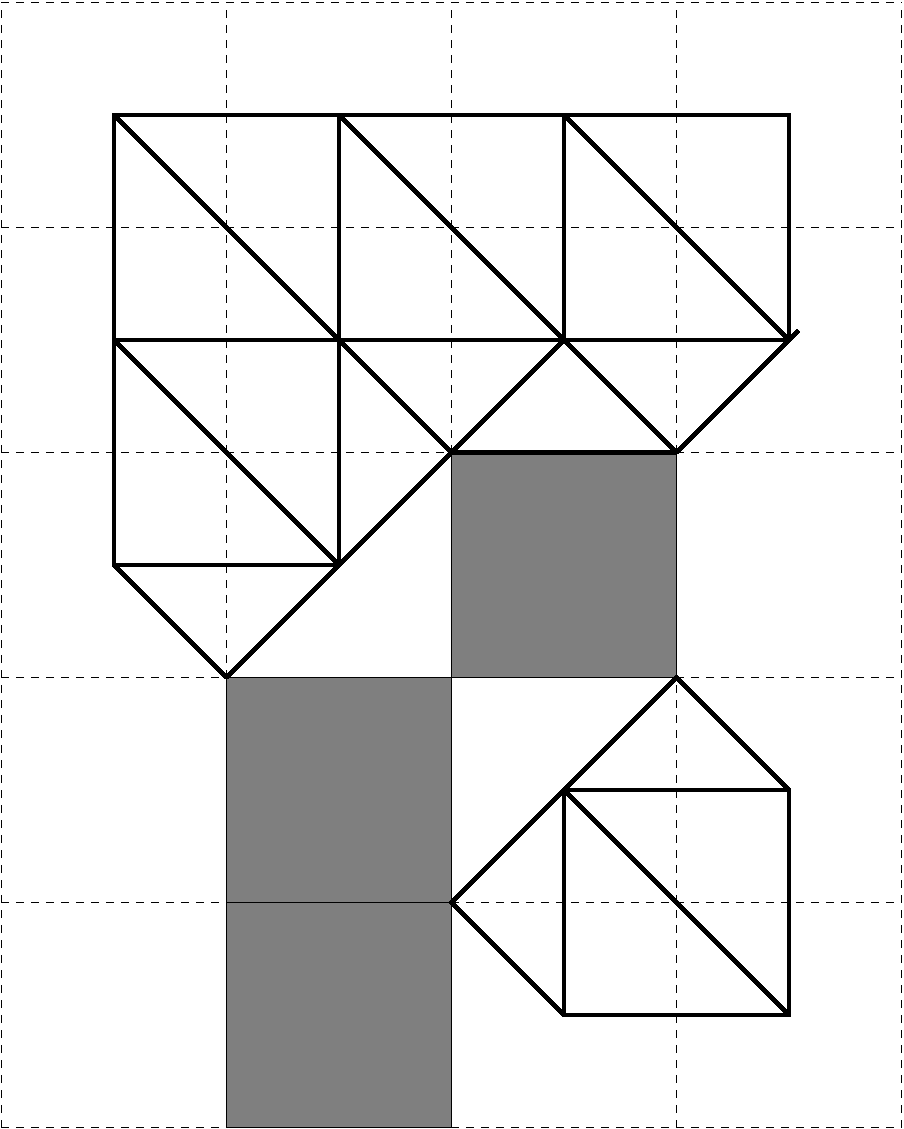
\includegraphics{FIG_wave/Subdiv_isthmus.pdf}}}\par
\end{minipage}
\begin{minipage}{3.2cm}
\centering
\rotatebox{90}{\resizebox{2.5cm}{!}{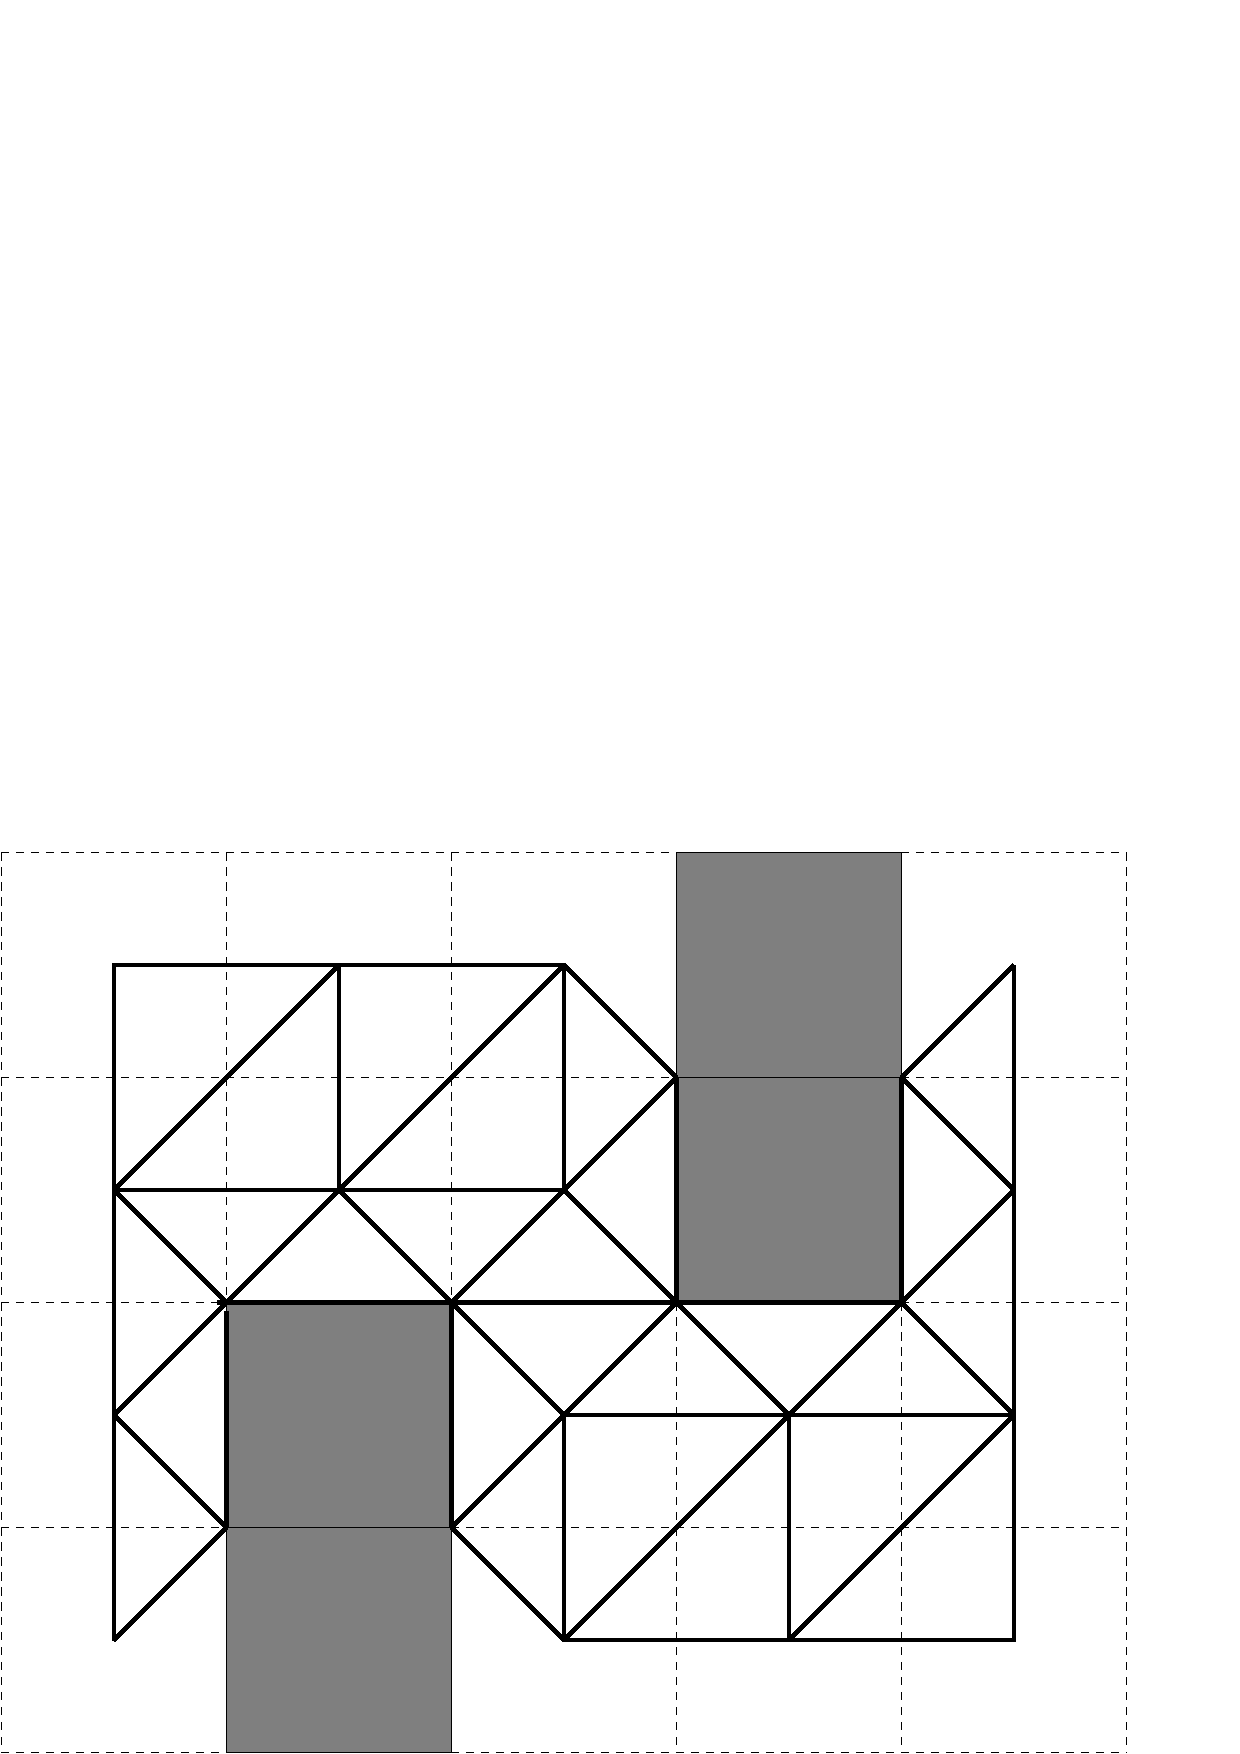
\includegraphics{FIG_wave/Subdiv_strait.pdf}}}\par
\end{minipage}
\end{center}
\item But the system also allows some finite element grid to be used.
\end{itemize}
}



\frame{
  \frametitle{The bump idealized test case}
We consider a shoaling test case on depth $4$ to $6$m and incoming waves of $1.02$m induce a current.
\begin{center}
\begin{minipage}{5.0cm}
\centering
\resizebox{4.4cm}{!}{\includegraphics{FIG_wave/Bennis_second_test/Hsignificant19501.png}}\par
\end{minipage}
\begin{minipage}{5.3cm}
\centering
\resizebox{4.4cm}{!}{\includegraphics{FIG_wave/Bennis_second_test/Vmagnitude_w19501.png}}\par
\end{minipage}
\end{center}
The total flux $(h+\xi)(\overline{v} + \overline{v}_s)$ is constant over the domain.
But the quantity $(h+\xi)\overline{v}_s$ is not constant over the domain even assuming no dissipation. The balanced $\divt {\bf u}_s=0$ is realized by the flux of $w_s$ at the surface, which is balanced by the flux of $w$.
}






\frame{
  \frametitle{Shoaling idealized test case I}
\begin{itemize}
\item For the shoaling idealized test case, a wave of period $1.5s$ arrives on a beach and breaks:
\begin{center}
\begin{minipage}{9.2cm}
\centering
\resizebox{7.0cm}{!}{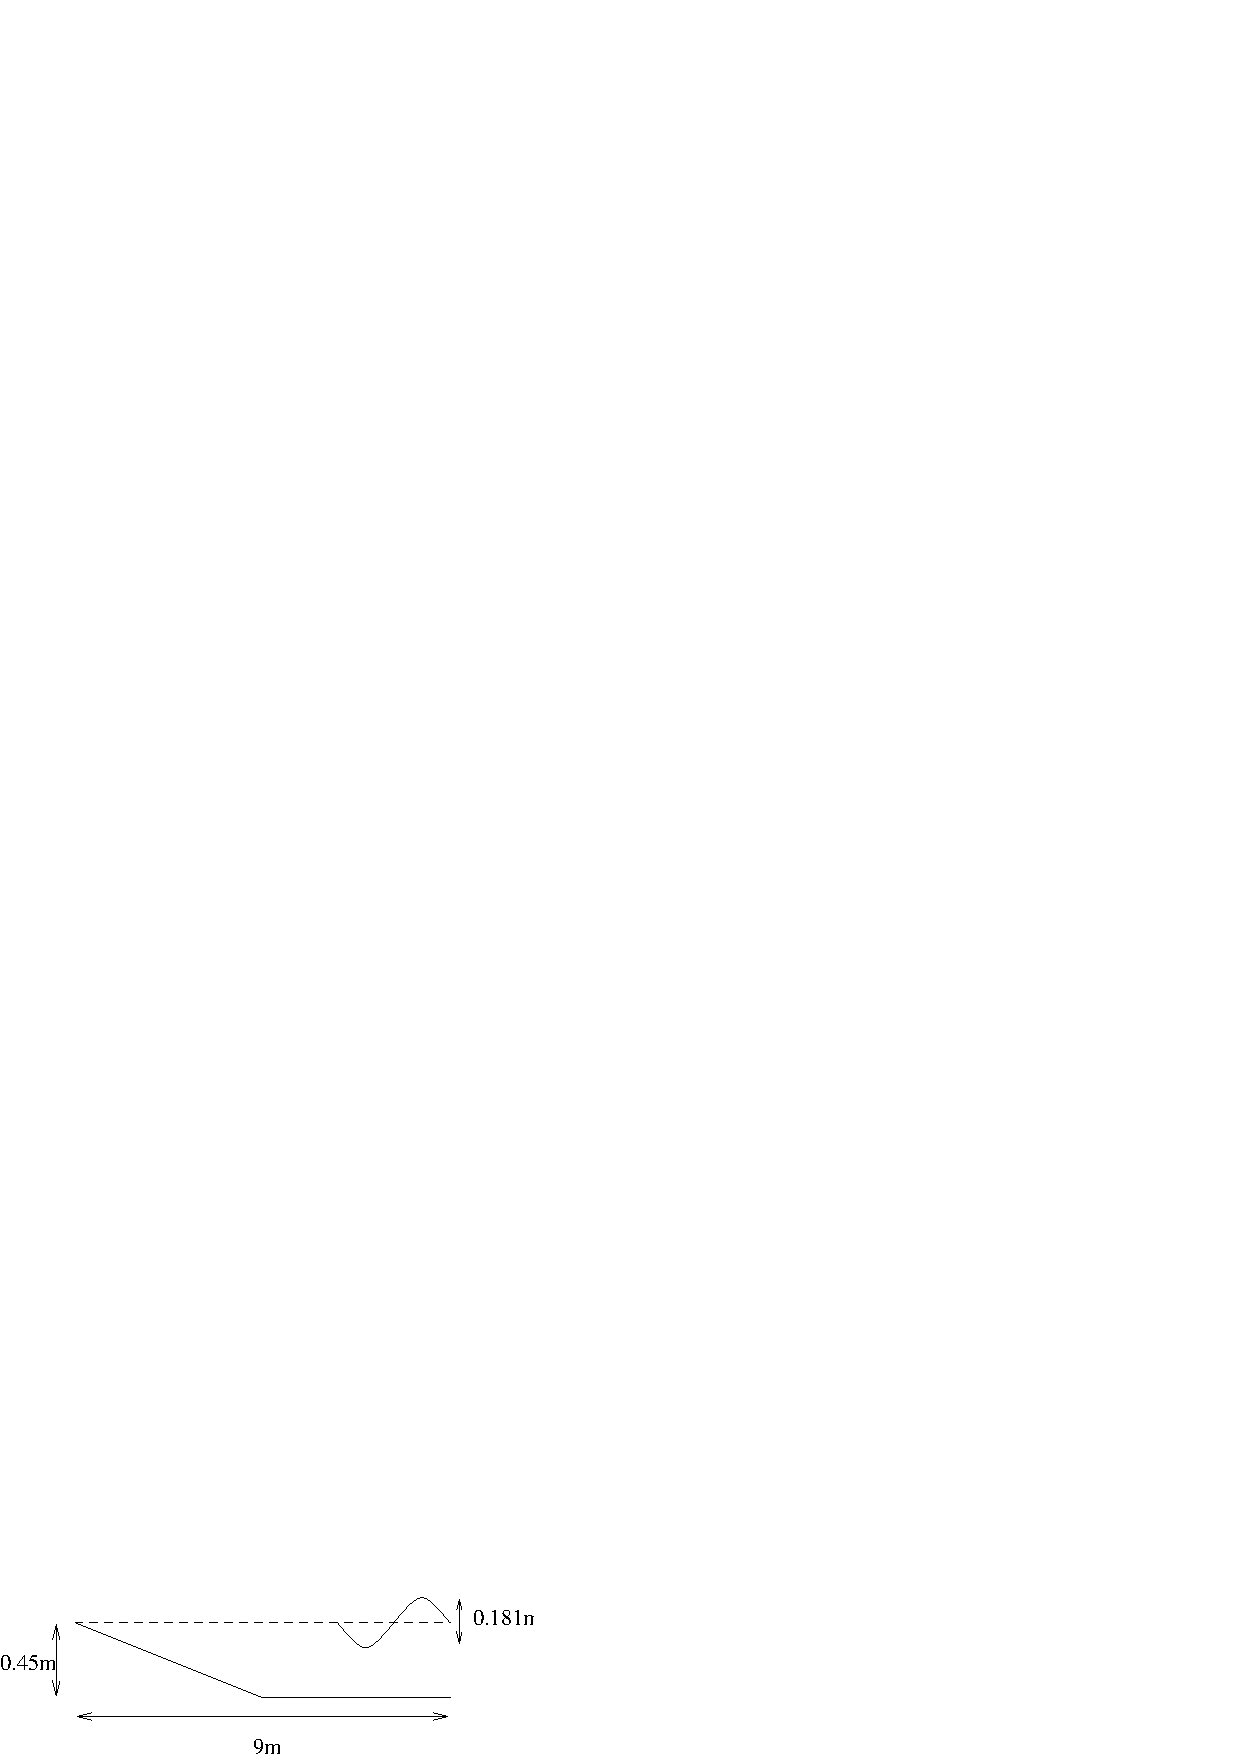
\includegraphics{FIG_wave/XIAsetup.pdf}}\par
\end{minipage}
\end{center}
\item The significant wave height satisfies to the two constraints:
\begin{equation*}
\begin{array}{rcl}
H_S^2 c_g  &=& Cst\mbox{~if~no~wave~energy~dissipation},\\
H_S & \leq & c_B (h +z) \mbox{~with~} c_B = 0.415.
\end{array}
\end{equation*}
\item The stress balance equation is
\begin{equation*}
\frac{\partial S_{xx}}{\partial x} = - \frac{1}{h+z} \frac{\partial h}{\partial x}
\end{equation*}
with $S_{xx}$ the Longuet-Higgins potential, $h$ the depth and $z$ the free surface.
\item The equation system can be solved very accurately.
\end{itemize}
}





\frame{
  \frametitle{Shoaling idealized test case II}
\begin{center}
\begin{minipage}{5.2cm}
\centering
\resizebox{5.0cm}{!}{\includegraphics[trim=15mm 5mm 15mm 10mm, clip]{FIG_wave/Zeta.png}}\par
Free surface
\end{minipage}
\begin{minipage}{5.2cm}
\centering
\resizebox{5.0cm}{!}{\includegraphics[trim=15mm 5mm 15mm 10mm, clip]{FIG_wave/Hsignificant.png}}\par
Significant wave height
\end{minipage}
\begin{minipage}{10.2cm}
\centering
\resizebox{10.0cm}{!}{\includegraphics[trim=15mm 5mm 15mm 10mm, clip]{FIG_wave/Lwave.png}}\par
Wave length
\end{minipage}
\end{center}
}


\frame{
  \frametitle{Visser's idealized test case}
\begin{itemize}
\item Another important test case is Visser's test case where the waves are arriving obliquely on the beach. A longshore current is induced by the waves and it is balanced by dissipation in the model.
\item In order to adequately model such situations, we introduce ideal grid, that is grids where the model does not see the whole coordinate system:
\begin{itemize}
\item Input contains triangle area, list of nodes and node depth.
\item Differences of coordinates between nodes of each triangles.
\end{itemize}
Everything (angle masks, differentials, ...) can be computed from this grid data.
\item This allows to build periodic grids for coupled wave models and so to simulate academic test cases with the coupled system.
\item When the model is in steady state a longshore current is induced by the waves and this current is balanced by dissipation in the model. See below results for Longuet-Higgins formulation:
\end{itemize}
\begin{center}
\begin{minipage}[t]{5.5cm}
\centering
\resizebox{4.5cm}{!}{\includegraphics[trim=15mm 10mm 15mm 10mm, clip]{FIG_wave/PictureVisser/Umagnitude.png}}\par
Longshore current
\end{minipage}
\end{center}

\begin{center}
\begin{minipage}[t]{10.5cm}
\centering
\resizebox{10.0cm}{!}{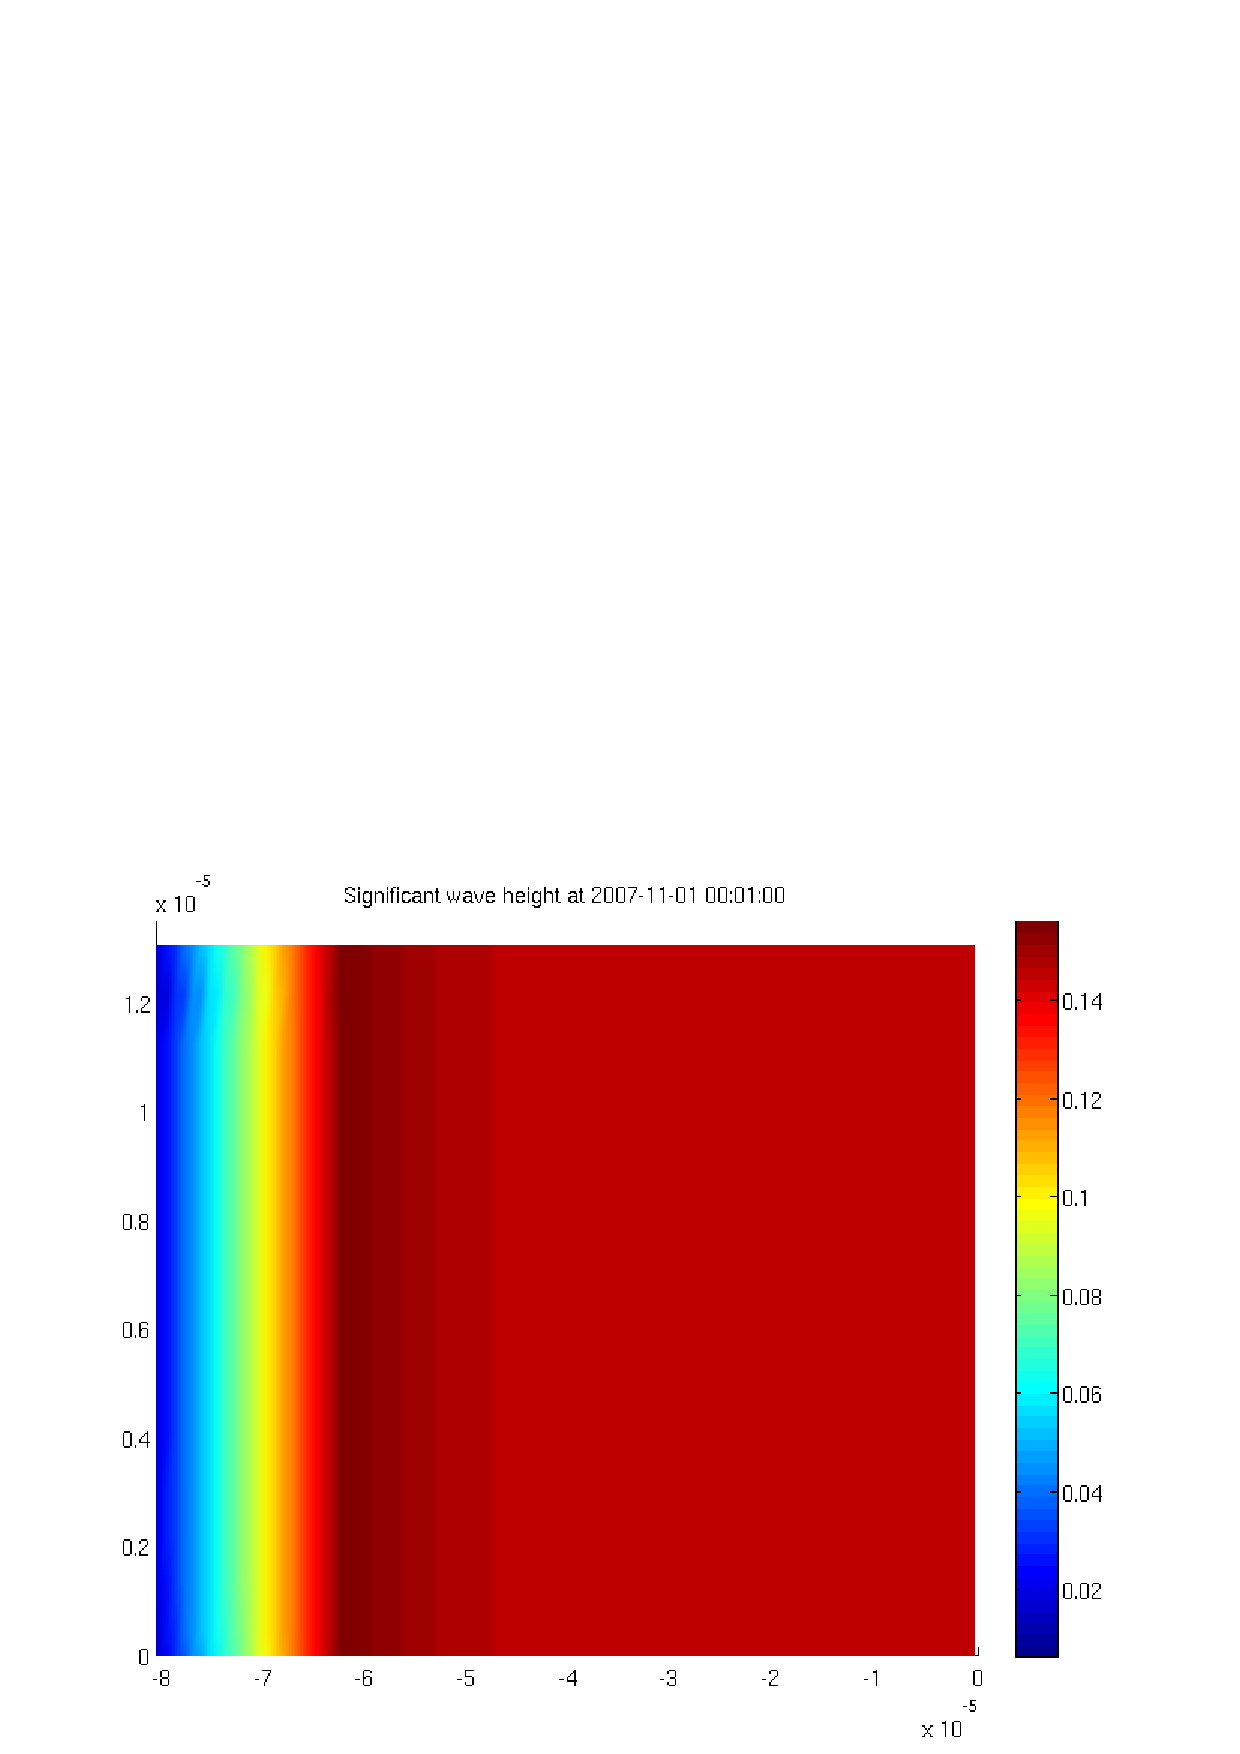
\includegraphics[trim=20mm 10mm 15mm 10mm, clip]{FIG_wave/PictureVisser/Hwave61_20071101_000100.png}}\par
Significant wave height
\end{minipage}
\begin{minipage}[t]{10.5cm}
\centering
\resizebox{10.0cm}{!}{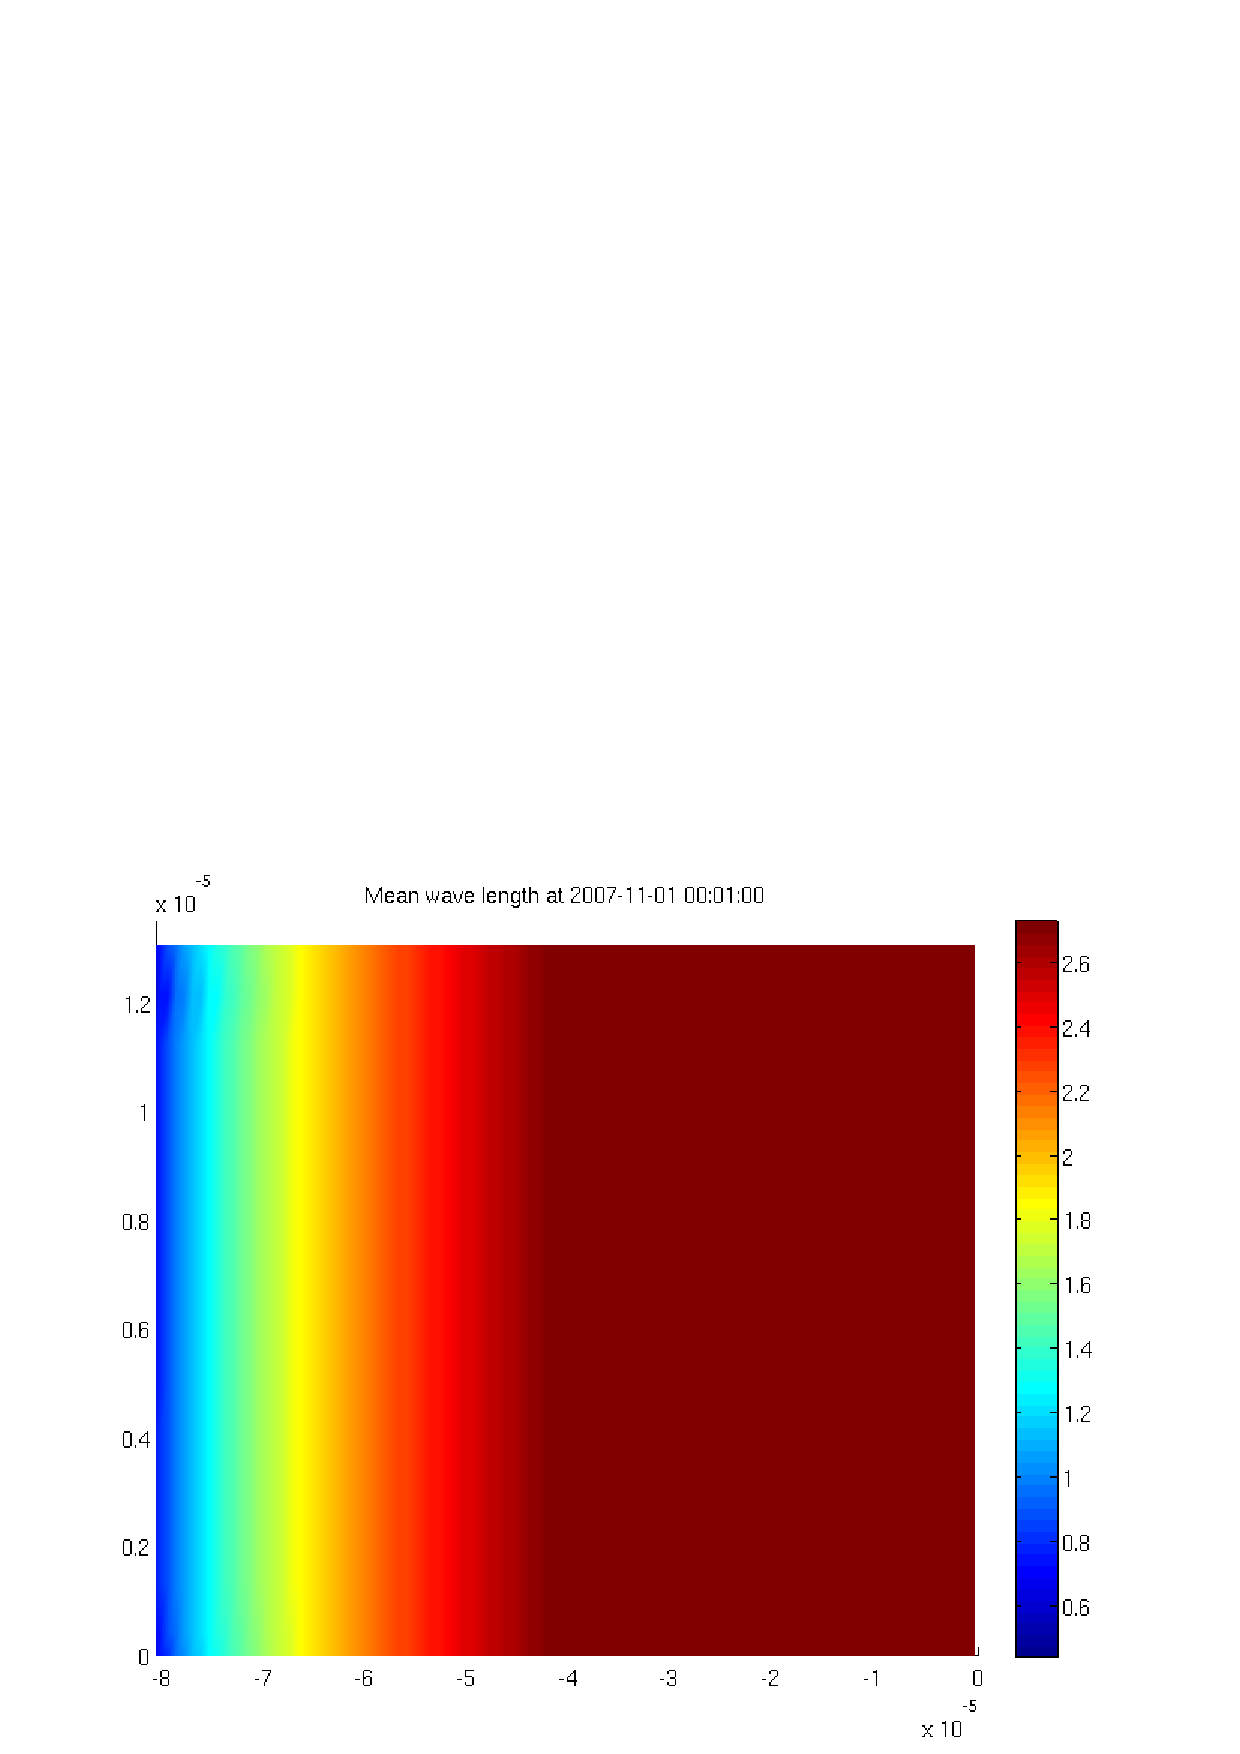
\includegraphics[trim=20mm 10mm 15mm 10mm, clip]{FIG_wave/PictureVisser/Lwave61_20071101_000100.png}}\par
Wave length
\end{minipage}
\begin{minipage}[t]{10.5cm}
\centering
\resizebox{10.0cm}{!}{\includegraphics[trim=15mm 10mm 15mm 10mm, clip]{FIG_wave/PictureVisser/Umagnitude.png}}\par
Longshore current
\end{minipage}
\begin{minipage}[t]{10.5cm}
\centering
\resizebox{10.0cm}{!}{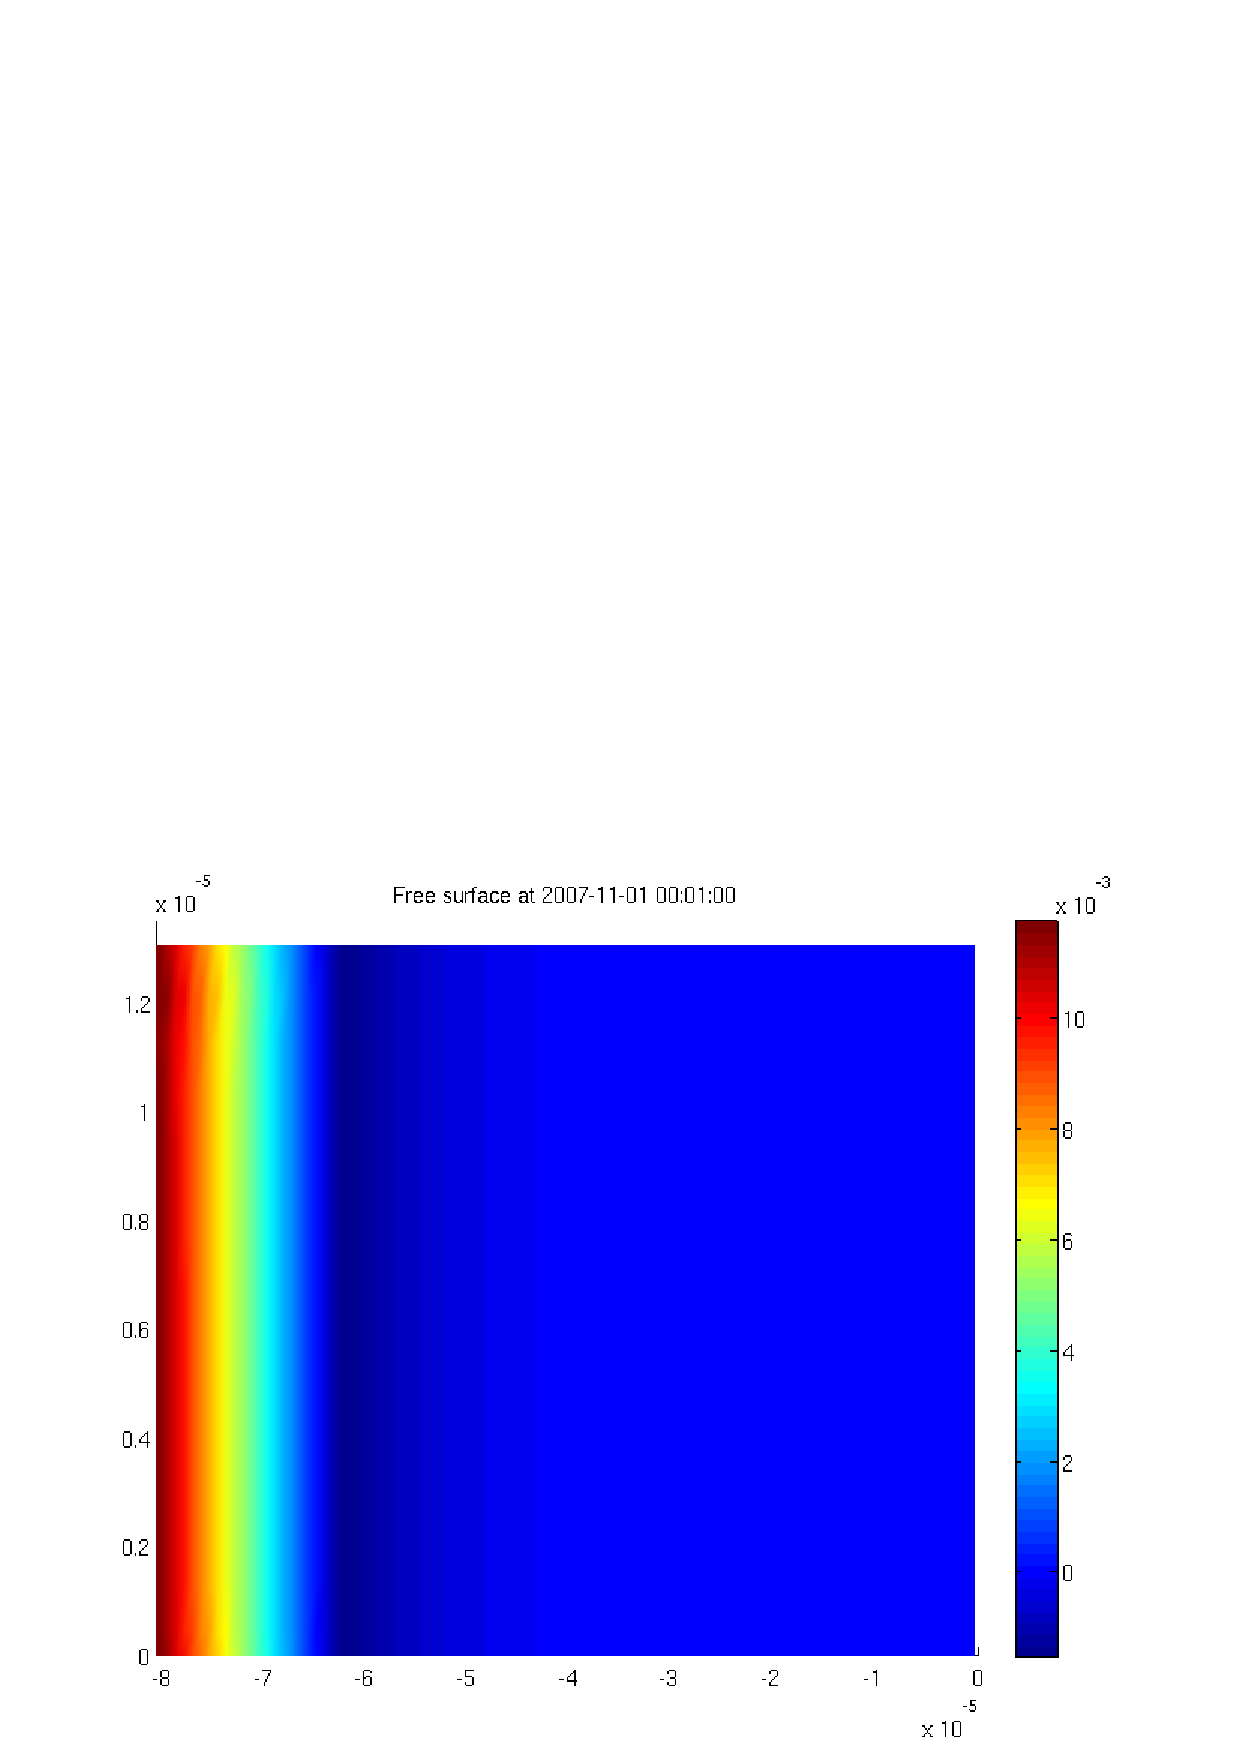
\includegraphics[trim=20mm 10mm 15mm 10mm, clip]{FIG_wave/PictureVisser/Zeta61_20071101_000100.png}}\par
Free surface
\end{minipage}
\end{center}
}
